\chapter{Research Methodology}

The purpose of this chapter is to introduce the research methodology, the
justification for using particular research methods used in this experimental
study on dimensional speech emotion recognition by fusing acoustic and
linguistic information. This approach allows the examination of the
contribution of fusing bimodal information for more accurate dimensional speech
emotion recognition. The research issues and philosophies used to tackle these
issues are discussed in this chapter. The implementation of research philosophy
through research strategies are highlighted. The experimental methods,
including datasets and an evaluation metric, are also the primary components of
the research methodology presented to close this chapter.

\section{Research motivation}
\subsection{Why is SER difficult?}
Speech emotion recognition (SER) is a difficult task. It differs from other
traditional tasks like image recognition (cat vs. dog), digit recognition, or
speech recognition. For instance, the features and labels for recognizing cat
or dog in image recognition are both clear. The difference in eyes, ears, skin
color, and shape between cat and dog can be used as informative features. The
labels also clear, either cat or dog, with a very high level of confidence. The
digit recognition problem has similar properties; from zero to nine can be
distinguished by their shapes; this input feature is an important factor for
the obtaining high accuracy classification.  Automatic speech recognition (ASR)
also has similar properties to both cases. SER is different from both cases.   

In SER, both features and labels are not clear. Researchers have attempted to
find useful features related to affective states (e.g.,
\cite{Batliner2011,Mairano}). In annotating labels for categorical or
dimensional emotion, the datasets makers rely on subjective evaluation. This
means that the labels are not exact values (e.g., compared to image labels).
However, high agreements among evaluators show the reliability of the datasets.
In this SER problem, it is almost impossible to obtain perfect accuracy, which
is possible to obtain in the previous image recognition problems.

\subsection{Why study dimensional SER?}
% argue with Darwin position
While most SER research focus on categorical emotion recognition, only a few
focuses on dimensional SER. In contrast, the present evidence about the
``fingerprint'' in categorical emotion, particularly based on facial
expression, is weak \cite{Barrett2019}. As Darwin argued that biological
categories, including emotion categories, does not have an essence due to the
high variability of individuals \cite{charles1872expression}, so does emotion
categories. 

Dimensional emotion may represent humans' affective state better than
categorical emotion. Humans do not perceive emotion categorically but in
continuous space. In this case, Russel argued that emotion categories could be
derived from valence-arousal space \cite{Russel1980}. Given this understanding,
dimensional SER is more challenging (since it predicts degree) and more useful
(since categorical emotion also can be derived) than categorical emotion
recognition.

% adding supporting research from "four not six" adding supporting factor from
% newest emotion model

\subsection{Why fuse acoustic with linguistic information?}
The third motivation is about the use of linguistic information. The simplest
answer to this question is that linguistic information is also can be extracted
from speech, and language is related to emotion. In other words, two pieces of
information can be extracted from speech without adding other modalities to
recognize expressed emotion. Hence, fusing acoustic and linguistic information
is reasonable and feasible for future SER implementation.

% other reasons: human multimodal processing and sentiment analysis
There are other possible motivations for fusing acoustic and linguistic
information for dimensional SER. One is from human multimodal processing, which
uses linguistic information as a cue for emotion perception
\cite{Lindquist2006}.  Another reason is that linguistic information is widely
used in sentiment analysis tasks, which are closely related to emotion
recognition. Sentiment analysis can be viewed as emotion recognition in text,
which focuses on sentiment or valence prediction.

% speech is basic need and may less private than image and video Speech is the
% most fundamental way to communicate. People use their voice to communicate,
% share experience, exchange ideas or transmit knowledge
% \cite{denes1993speech}. In some cases, people cannot avoid using speech to
% solve their urgent needs, e.g., complaining about a problem or calling a
% relation or a call center. Due to this necessity (to communicate with
% others), speech (acoustic and linguistic information) may less private than
% image or video data. 

In the speech chain, acoustic and linguistic are connected by a physiological
mechanism \cite{denes1993speech}. This chain shows a direct correlation between
linguistic and acoustic information. Fusing both pieces of information may
improve the prediction of the conveyed message. Since the message is elicited
from the same sources (e.g., thought, information, including emotion), using
both pieces of information is a straightforward way to track the transported
information, in this case, the expressed emotion of a speaker.

\section{Research issues}
% all issues
There are five issues discussed in this dissertation. The issues appeared from
the previous SER studies \cite{ElAyadi2011, Li2019b}. These issues raised in SER
from acoustic information, dimensional SER, and multimodal SER. Although these
issues are important, the previous chapter on literature study has found no
thorough study investigated on these five issues. The importance of these issues
and the contributions of this study to these issues are summarized below.

The first issue is the region of analysis used for feature extraction in
dimensional SER, local areas in frames, or whole utterance processing. The
importance of addressing this issue is to determine which region of analysis is
informative to extract dimensional emotion from speech. The
traditional way to extract acoustic features in acoustical signal processing is
frame-based processing. In this way, an utterance is split into several frames
in a fixed duration, e.g., 25 ms. A window function applies to these frames,
and the intended acoustic features are extracted on these frames. This local
feature extraction is known as a low-level descriptor (LLD). In contrast, the
newer research on speech emotion recognition proposed to extract statistical
functions based on these LLDs. These global features are known as high-level
statistical function (HSF). Form both features, it is unclear which one
performs better; one claimed that LLDs are enough since it is highly correlated
with emotion (e.g., tone and prosody \cite{Fritz2016}), others claimed that
global features are better in classification accuracy and classification time
(perhaps due to small feature size) \cite {ElAyadi2011}. This study revealed the
significant contribution of specific method for solving the effectiveness of
region analysis for acoustic feature extraction.

The second issue is the effect of the silence region in dimensional speech
emotion recognition. This issue is important to know whether such
post-processing techniques contribute to dimensional SER. In conventional ways,
acoustic features are extracted from speech utterance, including the silence
region. Some removed silence before extracting acoustic features (e.g.,
\cite{Atmaja2019, Elbarougy2019, Mairano, Aguilar2020}) and some used silence
as a feature (e.g., \cite{Atmaja2020f, Tian2015a}) or as an emotion category
\cite{Fayek2017}. Although silent pause is an important cue for human speech
communication \cite{Ephratt2008, Tisljar-Szabo2014}, it is unclear whether
silence contributes to human-computer communication (HCI). This study
contributed to this effect of silent pause region by predicting the role of the
region to dimensional SER.

The third issue is the low score of valence prediction in dimensional SER.
Among the three emotion dimensions, valence always obtained lower scores than
arousal and dominance. The previous study confirms this evidence
\cite{Li2019b}.  Considering valence is the most important emotion dimension
\cite{Fontaine2017}, the need to improve valence prediction score is worthwhile
to study. Although there are several attempts to improve valence prediction
\cite{Zhang2019, Aldeneh2017,Sridhar2018}, the obtained scores are still not
comparable to the scores achieved by arousal and dominance (e.g., in
\cite{Sridhar2018}). This study proposed and discussed a method to double the
performance of valence prediction in dimensional SER.

The fourth issue is whether it suffices to use acoustic features for modeling
emotions or if it is necessary to fuse them with linguistic features. Since
linguistic information can be obtained from speech (via ASR), it is reasonable
to fuse linguistic information with acoustic information. In HCI, the simplest
method to fuse multimodal information is by concatenating input features from
all modalities. More improvisation can be performed by concatenating models
instead of features. In other study, it was found that linguistic information
helps to improve valence prediction \cite{Karadogan2012}. Fusing acoustic and
linguistic information may improve not only valence prediction but also other
emotion dimensions. This study reveals the necessity of fusing both acoustic
and linguistic information for dimensional SER.

The fifth issue is the scheme or framework to fuse linguistic and acoustic
information. If the linguistic information contributes to dimensional emotion
prediction, what the most appropriate approach to fuse acoustic and linguistic
information is. In human multimodal emotion perception, how multimodal
information are fused is not clear yet. Both acoustic and linguistic
information are believed to be processed separately in different regions of the
cortex (right and left hemisphere). This mechanism inspires the late fusion
approach by processing each modality separately and fusing both results at the
decision level. This study showed the effectiveness of late fusion approach
over early fusion approach for combining acoustic and linguistic information
for dimension SER.


\section{Research philosophy}
Research philosophy can be defined as ``a belief about the way in which data
about a phenomenon should be gathered, analyzed and used \cite{Davison1998}."
This research used data-information-knowledge hierarchy (DIK) concept, which is
known as the canon of information science \cite{Fricke2009}. Figure
\ref{fig:research_concept} shows this DIK concept and its representation in the
speech emotion recognition area. Although some researchers defined these
concepts in different ways \cite{Badia2013, Liu2013}, the following concepts
are the proper and valid explanation used in this research.
% Human multimodal information fusion is unclear until now

% Human emotion perception The human ability to imagine situations in detail
% comes from the right hemisphere of the cortex, which approaches the world
% differently than the analytical, verbal left hemisphere. The right hemi-
% sphere is nonverbal and processes things in more holistic, integrated ways.
% It helps us see patterns, recognize faces, and identify and express emotions
% (Rewriting ...)

% change the picture to triangle (DIK) with its representation Speech, Acoustic
% + Linguistic, Emotion

% \subsection{}
\begin{figure}[htbp]
    \centering
    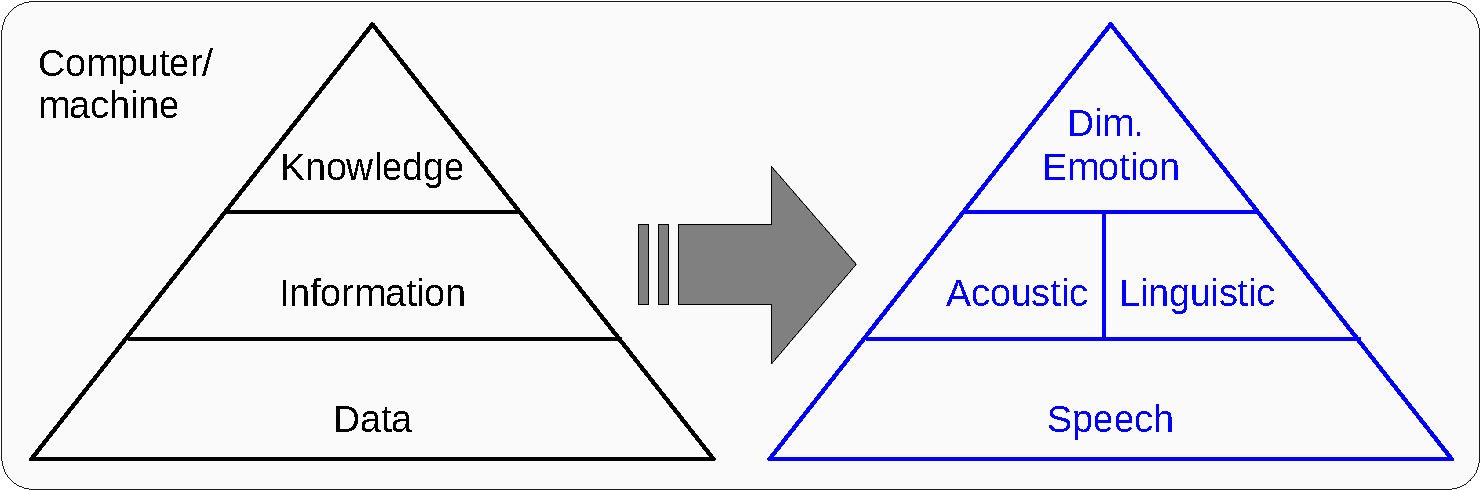
\includegraphics[width=.8\textwidth]{../fig/DIK_SER-crop.pdf}
    % \caption{A concept used in this research: acoustic and linguistic
    % information are extracted from (speech) data to obtain knowledge -- the
    % dimensional emotion.}
\caption{The DIK hierarchy and its representation in speech emotion
recognition; information (I) is extracted from data (D); knowledge (K) is
extracted from information.}
    \label{fig:research_concept}
\end{figure}

\subsubsection{Data: speech}
Data is worth nothing. According to Choo \cite{Choo2007}, signals structure the
data. Acoustic signal composes speech; speech is the data. In human
communication, speech by a speaker is data for the listener. In HCI, the speech
dataset is a collection of recorded utterances from speakers elicited intended
expressions. An emotional speech dataset is a type of speech dataset that
provides utterances with their emotional labels in categorical or/and
dimensional emotions.

\subsubsection{Information: acoustic and linguistic}
Information is know-what. It is the relevant, usable, significant, meaningful,
or processed data \cite{Rowley2007}. Information is extracted from data. Humans
arguably perceive the speaker's emotions from their acoustic and linguistic
information \cite{Nygaard2008}. How both pieces of information fused is not
clear until now; however, researchers suggest that both perceived information
are processed separately \cite{Berckmoes2004, Kotz2011}, verbal information in
the left cortex and non-verbal information in the right cortex. In HCI,
acoustic information can be extracted directly from speech, while linguistic
information needs a mediator, i.e., speech-to-text system, to extract words
from speech. Then, linguistic information can be extracted from these words.
Both pieces of information are represented as features. Feature extraction is
the process of extracting acoustic and linguistic information from the speech
dataset and its transcription.

\subsubsection{Knowledge: dimensional emotion degrees}
Knowledge is know-how. It is extracted from the information. Knowledge
transforms information into instructions. In human communication, the knowledge
to perceive emotion is innate rather than learned \cite{Matsumoto2009}. In
dimensional emotion, the outputs of this knowledge are the degrees of valence
(V), arousal (A), and dominance (D) [e.g., V=4, A=4, D=2]. The process of
mapping information (features) to dimensional emotion degree is a regression
task which is performed by such regressors. 

\section{Research strategy}
A research strategy is the steps or ways in which research's goals could be
achieved. The goal of this study is to answer the research issues presented
previously. This research investigates three strategies to answers these
research issues. The following are the description and rationale of the
strategies.

% outline three proposed methods, which methods to tackle which issues
\subsection{Dimensional SER by acoustic information}
This study evaluated dimensional SER based on acoustic features to tackle the
first and second issues.  This study aims at maximizing the potency of
acoustic-based SER. First, the region of analysis is investigated. A thorough
comparison among three conditions are performed: (1) extracting acoustic
features from silence-removed regions, (2) extracting acoustic features from
the whole region, including silence, and (3) extracting features from the whole
region and utilizing a silence feature as an additional feature. Second, this
study evaluated which aggregation method performs better: input features
aggregation or outputs aggregation. The common approach in aggregation is
output aggregation by majority voting; however, input aggregation may perform
better, particularly dimensional SER. For instance, humans may perceive emotion
from acoustic information aggregation (e.g., tones) to recognize the emotion
based on that information (rather than aggregating emotions/outputs). As found
in other SER research, this study contributes to the necessity to go beyond
acoustic-only SER.

% add fictitious case where linguistics may helps
\subsection{Fusing acoustic and linguistic information at feature level}
In certain cases, it may be difficult for a listener to perceive the speaker's
emotion from acoustic information only. For instance, both joy and angry may
have a similar intonation (e.g., high tones); hence it is difficult to
differentiate both emotions. By knowing the semantic of utterances, it may be
easier to judge the expressed emotion for both human-human communication and
human-computer communication.  This case raises an opportunity to investigate
whether linguistic information contributes to dimensional emotion recognition.
Although the study of this phenomenon has been performed previously (e.g., in
\cite{Karadogan2012}), several limitations still exist. The emotion model, the
used linguistic information, and the classification framework have evolved
since the publication.

Apart from the need for multimodal/bimodal information fusion, linguistic
information has been actively developed for sentiment analysis, analyzing text
to obtain the affective state of the writer (positive or negative).  This
`sentiment' term reflects directly to valence; hence, one possible solution to
improve low valence score in dimensional SER is by utilizing linguistic
information. Research showed that utilizing linguistic information improves
both categorical {\cite{ Yoon2018} and dimensional \cite{Karadogan2012} emotion
recognitions. Fusing acoustic and linguistic information tackles both the third
and fourth issues: the low score valence prediction and the necessity of using linguistic information.

A simple approach to fuse acoustic and linguistic information is by fusing both
at the feature level. In this approach, either features or networks can be
concatenated to predict dimensional emotions. In the first method, all features
are inputted to the same classifier, while in the latter, both pieces of
information may have different classifiers (networks). In the latter method,
additional networks are needed to fuse both networks, typically a type of dense
networks (also called as fully connected [FC] networks or multilayer perceptron
[MLP]).

Although there are several studies that focus on the linguistic and acoustic
features fusion for SER at the feature level, this study differs in several
aspects. First, this study evaluated both feature concatenation and network
concatenation. Second, this study proposed correlation-based multitask learning
(MTL) to predict valence, arousal, and simultaneously from both acoustic and
linguistic information. Third, this study contributes to a comparison of manual
and automatic transcriptions for acoustic-linguistic dimensional SER.

\subsection{Fusing acoustic and linguistic information at decision level}
To extend the fourth issue, it is necessary to study the fusion of acoustic and
linguistic information not only at the feature level but also at the decision
level. This strategy is motivated by human multimodal processing. The neural
mechanism on how the brain processes multimodal information suggests that each
information is processed in a separate brain region. Hence, a late fusion
approach, i.e., decision-level information fusion, may work better than
feature-level fusion. Apart from investigating which fusion method is better to
combine bimodal information (the fifth issue), this strategy can also be used
to investigate the third and fourth issues.

This last strategy contributes to investigate which framework performs better
for fusing acoustic and linguistic information. Although there is an argument
that any fusion approach will perform similarly \cite{Pepino2020}, the opposite
also has been argued \cite{Planet2012}. Consistency found in this study (that
late fusion is better than early fusion) may help the future research on
dimensional SER and trigger more ways to fuse both acoustic and linguistic
information for SER.

% \section{Experiments}
\section{Datasets}
The strategies to answer research issues need several instruments to experiment
with. One key component in this dimensional SER research is dataset. Three
emotional speech datasets have been chosen for different experiments. These
three datasets are explained below. \\

% explain three datasets and their partition
\noindent 1. IEMOCAP \\
IEMOCAP, which stands for interactive emotional dyadic motion capture database,
contains dyadic conversations with markers on the face, head, and hands. The
recordings thus provide detailed information about the actors's facial
expressions and hand movements during both scripted and spontaneous spoken
communication scenarios \cite{Busso2008}. This research only uses acoustic and
linguistic features because the goal is bimodal speech emotion recognition. The
IEMOCAP dataset is freely available upon request, including its labels for
categorical and dimensional emotions. This study uses dimensional emotion labels
(valence, arousal, dominance), which are average scores for two evaluators,
because they enable deeper emotional states analysis. The dimensional emotion
scores, for valence, arousal, and dominance, are meant to range from 1 to 5 as
a result of Self-Assessment Manikin (SAM) evaluation. It has been found that
some labels with scores lower than 1 or higher than 5. Either removing those
data (seven samples) or converting them into neutral (a score of 3) was chosen
in different experiments.  All labels are then converted from the 5-point scale
to a floating-point values range [-1, 1] when fed to a DNN system.

The total length of the IEMOCAP dataset is about 12 hours, or 10039
turns/utterances, from ten actors in five dyadic sessions (two actors each).
The speech modality used to extract acoustic features is a set of files in the
dataset with a single channel per sentence. The sampling rate of the speech
data was 16 kHz. The manual transcription in the dataset without additional
preprocessing is used for text data except for comparing it with ASR outputs
(chapter 5). \\

\noindent 2. MSP-IMPROV \\
MSP-IMPROV \cite{busso2016msp}, developed by the Multimodal Signal Processing
(MSP) Lab at the University of Texas, Dallas, is a multimodal emotional
database obtained by applying lexical and emotion control in the recording
process while also promoting naturalness. The dataset provides audio and visual
recordings, while text transcriptions are obtained via automatic speech
recognition (ASR) provided by the authors of the dataset. As with IEMOCAP, the
speech and speech+text data with dimensional emotion labels were used in
different experiments. The annotation method for the recordings was the same as
for IEMOCAP, i.e., SAM evaluation, with rating by at least five evaluators.
Some data with missing evaluations were treated as neutral speech (i.e., a
score of 3 for valence, arousal, and dominance). Also, as with IEMOCAP, all
labels are converted to floating-point values in the range [-1, 1] from the
original 5-point scale.

The MSP-IMPROV dataset contains 8438 turns/utterances in more than 9 hours.
Similar to IEMOCAP, there are two speakers for each session. The number of
sessions is six. Originally, the dataset is divided into four scenarios:
``Target-improvised" and ``Target-read," ``Other-improvised," and
``Natural-interaction.'' This allotment was designed to evaluate the effect of
target sentences. The whole dataset is used for acoustic-only emotion
recognition. The parts of MSP-IMPROV, excluding ``Target-read," are used for
acoustic-linguistic information fusion. A further explanation about this
dataset will be added in the explanation of the experiment involving this
dataset (Chapter 6).\\

\noindent 3. USOMS-e \\
Ulm State of Mind in Speech-elderly (USOMS-e) dataset is the corpus used in the
elderly emotion sub-challenge in the INTERSPEECH 2020 computational
paralinguistic challenge. The whole dataset subset is used with 87 subjects
aged 60 -- 95 years; 55 of the subjects were male, and the rest 32 were female.
The dimensional emotion labels were given in valence and arousal divided into
three categories: low, medium, and high.

Table \ref{tab:dataset} shows the number of instances/stories and chunks in all
partitions. The labels are given per each story. The label on the dataset is
given on both alphabetic and numeric symbols, i.e., low ('L' or '0'), medium
('M' or '1'), and high ('H' or '2'). This research used alphabetic labels as
given in the baseline paper. Note that the number of chunks is different for
each story; for instance, there are 34 chunks in the first story and 46 chunks
in the second story.

\begin{table}[t]
  \caption{Number of instances and chunks in each partition USOMS-e dataset}
  \label{tab:dataset}
  \centering
  \begin{tabular}{ l c c }
    \hline
Partition & \# Stories (text) & \# Chunks (audio) \\
\hline \hline
Train     & 87                & 2496  \\
Dev       & 87                & 2466  \\
Test      & 87                & 2816  \\
    \hline
Total     & 261               & 7778 \\
    \hline
  \end{tabular}
  \end{table}


\section{Evaluation metric}
% explain CCC
Apart from the datasets, a metric to measure the performance of
proposed/evaluated methods is needed to evaluate the research. Instead of using
several metrics, this research focus on the use of concordance correlation
coefficient (CCC) as a single metric to evaluate the performance of dimensional
SER.  This metric is proposed to be the standard metric for dimensional SER
previously \cite{Ringeval2015a}. The formula to calculate CCC is given as, 
\begin{align} 
  CCC &= \dfrac{2 \rho \sigma_x \sigma_y} {\sigma_x^2 + \sigma_y^2 + (\mu_x - \mu_y)^2},
  % CCCL &= 1 - CCC
\end{align}
where $\rho$ is the Pearson correlation coefficient (PCC/CC) between predicted
emotion degree $x$ and true emotion degree $y$, $\sigma^2$ is a variance and
$\mu$ is a mean. This metric is more challenging than the correlation
coefficient since it penalizes the score, even the correlation is well but
shifted.  The penalized values are in proportion to the deviation.

\section{Summary}
This chapter presents the research methodology for studying dimensional SER by
fusing acoustic and linguistic information. The motivations to choose this
research theme are discussed, and the raised issues are presented. These five
issues are region of analysis for acoustic feature extraction, effect of silent
pause features, low valence prediction, the necessity for fusing acoustic with
linguistic information, and framework for fusing acoustic with linguistic
information. These issues have never been studied thoroughly in the previous
studies. The importance of each issue and the contribution of this study to
each issue are briefly described. Three strategies are highlighted to address
these issues, including the datasets to evaluate the strategies and a metric to
measure the performance. The proposed strategies investigate the necessity of
going beyond acoustic information and the necessity to fuse acoustic with
linguistic information for dimensional SER. The next three chapters 
discuss each strategy proposed in this chapter, followed by a chapter on
Comparative Analysis and a Conclusions chapter to end the discussion.
% Research's dataset Computational Unit \section{Summary}

% \newpage
% \thispagestyle{empty}
% \mbox{}
